\chapter{PENGUJIAN DAN ANALISIS}
\label{chap:pengujiananalisis}

% Ubah bagian-bagian berikut dengan isi dari pengujian dan analisis

Pada penelitian ini dipaparkan mengenai pengujian dari model yang dibuat pada metodologi sebelumnya. Hasil pengujian kemudian akan dianalisis dan diharapkan dari hasil analisis didapatkan kesimpulan mengenai model yang dibuat dengan metode yang telah ditentukan.

Hasil yang dibahas merupakan hasil dari proses dua dataset, yaitu; dataset dari mata uang USDCHF dengan jangka waktu 5 menit dengan total dataset 100.000 dan  dataset dari mata uang EURUSD dengan jangka waktu 15 menit dengan total dataset 50.104 . Model yang digunakan dan dibahas adalah model Time Series Transformer dan Long Short Term Memory dengan Timestep 12,24, dan 36.
\section{Pembahasan Hasil Pelatihan Dengan Mata Uang USDCHF}
Dari penelitian ini proses training dilakukan menggunakan beberapa parameter utama, yaitu jumlah epoch sebanyak 100, optimizer untuk memperbarui bobot model, dan fungsi loss (criterion) untuk menghitung selisih antara hasil prediksi dan target. Data dibagi ke dalam dua loader, yaitu train\_loader untuk proses training dan test\_loader untuk proses validasi, dengan ukuran batch yang ditentukan saat pembuatan data loader. Optimizer dan fungsi loss yang digunakan disesuaikan dengan jenis permasalahan dan arsitektur model. Selama proses training, model secara bertahap melakukan forward pass, backward pass, dan pembaruan parameter menggunakan optimizer. 

Proses Training dilakukan dengan time step yang bereda beda, yaitu: 12,24, dan 36 dengan hasil sebagai berikut
\begin{figure} [H] \centering
  % Nama dari file gambar yang diinputkan
    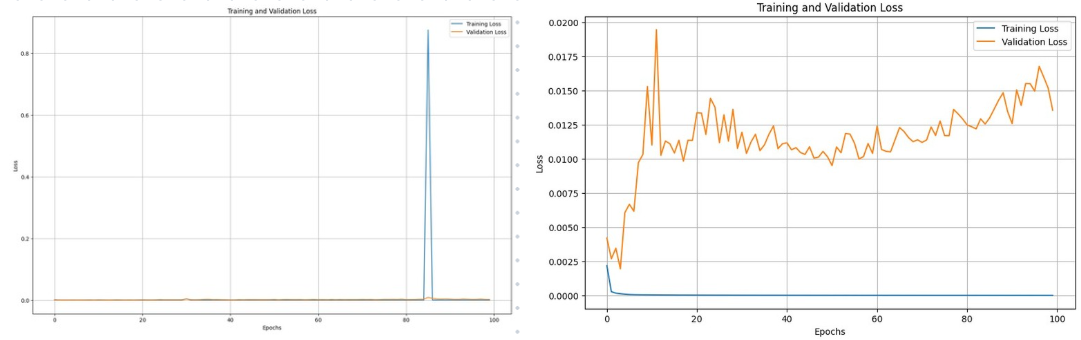
\includegraphics[scale=0.8]{gambar/perbandingan train(12).png} 
    \caption{Hasil Train Dengan Time Step 12}
    \label{fig:label_gambar}
\end{figure}
Pada timestep 12, grafik dari model Time Series Transformer menunjukkan adanya lonjakan yang cukup signifikan pada training loss yang mengalami lonjakan sangat tinggi di epoch ke - 85. Hal ini dapat disebabkan learning rate yang terlalu tinggi atau data yang ada dalam bacth tertentu yang mengalami penurunan atau kenaikan yang cukup signifikan sehingga berbeda dari data lainnya . Sementara itu, validation loss tetap berada pada nilai rendah dan stabil.

Berbeda dengan Time Series Transformer, model LSTM menunjukkan hasil yang lebih stabil. Training loss menurun hingga mendekati nol, sedangkan validation loss berada di atas training loss, namun masih dalam rentang nilai yang stabil. Kondisi ini mengindikasikan bahwa LSTM mampu mempelajari data training dengan baik, tetapi mulai menunjukkan tanda-tanda overfitting, karena terdapat gap antara training loss dan validation loss.

\begin{figure} [H] \centering
  % Nama dari file gambar yang diinputkan
    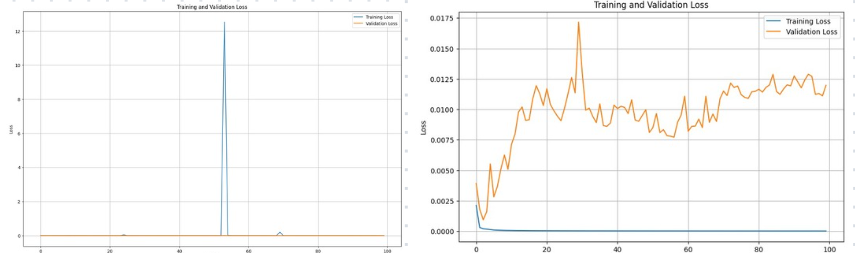
\includegraphics[scale=0.98]{gambar/perbandingan train(24).png} 
    \caption{Hasil Train Dengan Time Step 24}
    \label{fig:label_gambar}
\end{figure}

Pada Timestep 24,TST menghasilkan pola yang serupa dengan timestep 12, di mana training loss mengalami lonjakan di beberapa titik, tetapi menghasilkan grafik validation loss yang sangt baik dan stabil. Hal ini kembali menunjukkan model kesulitan dalam menjaga kestabilan training saat jumlah timestep bertambah.Sedangkan LSTM masih cukup stabil, meskipun validation loss sedikit lebih berfluktuasi dibandingkan saat timestep 12. Training loss tetap sangat rendah, dan terdapat tren validation loss yang sedikit naik seiring bertambahnya epoch, menandakan potensi overfitting yang mulai meningkat.


\begin{figure} [H] \centering
  % Nama dari file gambar yang diinputkan
    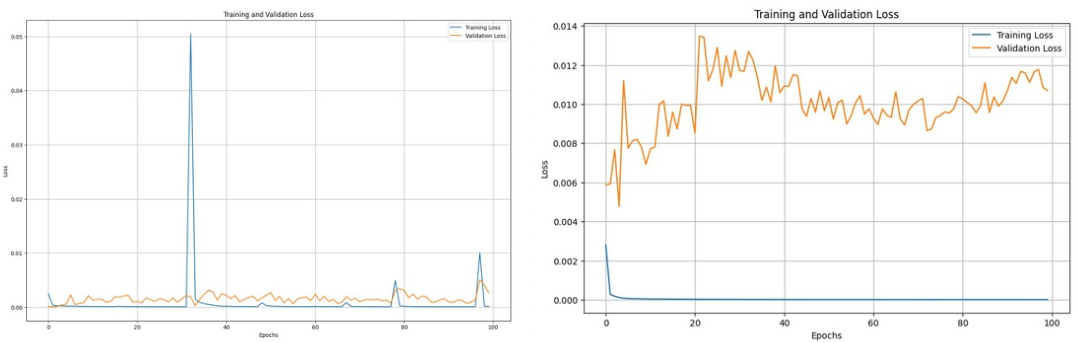
\includegraphics[scale=0.75]{gambar/perbandingan train(36).png} 
    \caption{Hasil Train Dengan Time Step 36}
    \label{fig:label_gambar}
\end{figure}
Pada timestep 36, Time Series Transformer menunjukkan sedikit perbaikan dibandingkan dengan timestep sebelumnya. Meskipun validation loss masih mengalami fluktuasi, frekuensi lonjakan ekstrem berkurang. Hal ini menunjukkan bahwa dengan window time series yang lebih panjang, model mulai dapat menangkap pola data dengan lebih baik, meskipun kestabilan training masih menjadi isu yang perlu diperbaiki.

Di sisi lain, model LSTM tetap konsisten dengan pola hasil sebelumnya. Training loss kembali mendekati nol, sementara validation loss cenderung stabil, meskipun terdapat kecenderungan peningkatan nilai di epoch-epoch akhir. Hal ini menguatkan indikasi bahwa model LSTM mulai mengalami overfitting saat jumlah timestep bertambah, karena model terlalu fokus pada data training dan kehilangan kemampuan generalisasi terhadap data validasi.

Berdasarkan hasil pelatihan kedua model dengan variasi timestep, dapat disimpulkan bahwa:
\begin{itemize}
    \item Time Series Transformer memiliki performa yang sensitif terhadap perubahan jumlah timestep. Validation loss sering kali mengalami lonjakan ekstrem, yang menandakan ketidakstabilan training.

    \item LSTM menunjukkan performa yang lebih stabil dan konsisten, meskipun terdapat kecenderungan overfitting saat jumlah timestep meningkat. Hal ini ditunjukkan dengan training loss yang sangat rendah, sementara validation loss relatif stagnan atau cenderung naik di epoch-epoch akhir.

\end{itemize}

\section{Pembahasan Hasil Pelatihan Dengan Mata Uang EURUSD}
Dari penelitian ini proses training dilakukan menggunakan beberapa parameter utama, yaitu jumlah epoch sebanyak 100, optimizer untuk memperbarui bobot model, dan fungsi loss(criterion) untuk menghitung selisih antara hasil prediksi dan target. Data dibagi ke dalam dua loader, yaitu train loader untuk proses training dan test loader untuk proses validasi, dengan
ukuran batch yang ditentukan saat pembuatan data loader. Optimizer dan fungsi loss yang digunakan disesuaikan dengan jenis permasalahan dan arsitektur model. Selama proses training, model secara bertahap melakukan forward pass, backward pass, dan pembaruan parameter menggunakan optimizer.
\begin{figure} [H] \centering
  % Nama dari file gambar yang diinputkan
    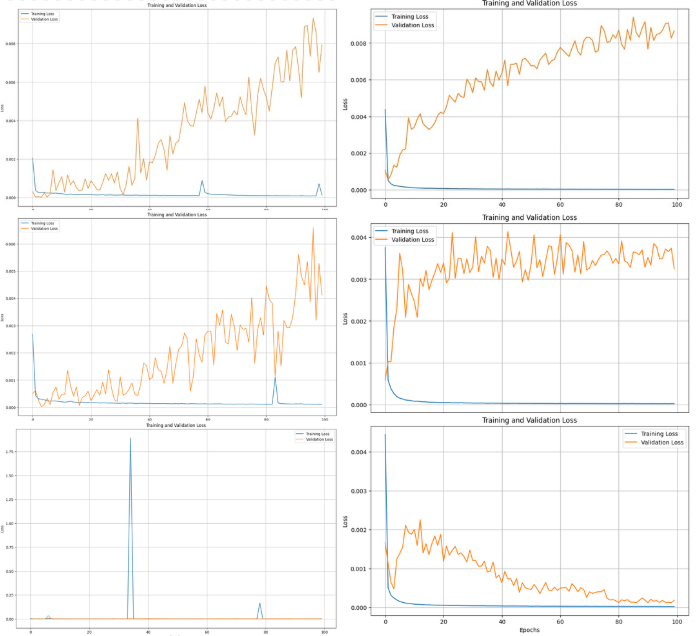
\includegraphics[scale=1.2]{gambar/perbandingan training_EURUSD.png} 
    \caption{Hasil Prediksi Harga Open Dengan Time Step 12}
    \label{fig:label_gambar}
\end{figure}
Gambar di atas memperlihatkan grafik Training Loss dan Validation Loss dari hasil pelatihan model Time Series Transformer (TST) (sebelah kiri) dan Long Short-Term Memory (LSTM) (sebelah kanan) pada data EUR/USD dengan variasi timestep 12, 24, dan 36 selama 100 epoch. Grafik ini berfungsi untuk mengevaluasi kestabilan dan kemampuan generalisasi masing-masing model selama proses pelatihan.

\subsection{Model Time Series Transformer (TST) – (Sebelah Kiri)}
\begin{itemize}
    \item \textbf{Timestep 12:}
    
    Training Loss turun cepat di awal dan stabil di nilai sangat rendah. Validation Loss juga relatif stabil tanpa lonjakan besar, menandakan proses pelatihan berjalan baik dan overfitting relatif minim.
    
    \item \textbf{Timestep 24:}
    
    TST kembali menunjukkan performa konvergensi yang baik. Training Loss tetap rendah sepanjang epoch, sementara Validation Loss berada di kisaran nilai tetap tanpa fluktuasi ekstrem, menandakan model mampu melakukan generalisasi yang lebih baik.

    
    \item \textbf{Timestep 36:}

    Performa terbaik ditunjukkan pada konfigurasi ini. Baik Training Loss maupun Validation Loss menurun dan stabil tanpa spike signifikan. TST berhasil menjaga kestabilan prediksi dan konvergensi dengan sangat baik pada timestep yang lebih panjang.
\end{itemize}

\subsection{Model LSTM – (Sebelah Kanan)}
\begin{itemize}
    \item \textbf{Timestep 12:}
    
    Training Loss turun drastis ke nilai sangat rendah di awal epoch. Namun, Validation Loss meningkat seiring bertambahnya epoch, dengan fluktuasi yang cukup besar. Pola ini menunjukkan indikasi overfitting, di mana model terlalu cocok terhadap data latih dan kurang baik dalam memprediksi data uji.
    
    \item \textbf{Timestep 24:}
    
    Masih ditemukan pola yang serupa. Training Loss stabil di nilai rendah, tetapi Validation Loss tetap fluktuatif dan cenderung naik, dengan beberapa spike. Hal ini mengindikasikan masalah overfitting yang masih terjadi meskipun panjang timestep bertambah.

    
    \item \textbf{Timestep 36:}

    Training Loss tetap rendah, sementara Validation Loss sedikit lebih stabil dibandingkan pada timestep sebelumnya. Meskipun demikian, gap antara Training Loss dan Validation Loss masih cukup besar, menandakan performa generalisasi LSTM belum optimal.
\end{itemize}

\section{Hasil Prediksi Mata Uang USDCHF}
\subsection{Hasil Prediksi Harga Open Dengan Timestep 12}
Pada grafik sebelah kiri, terlihat hasil prediksi harga open menggunakan model LSTM. Garis biru merepresentasikan harga aktual, sedangkan garis merah menunjukkan hasil prediksi. Secara umum, model LSTM mampu mengikuti pola pergerakan harga pasar modal dengan baik, di mana arah tren kenaikan dan penurunan harga berhasil diikuti oleh hasil prediksi.Namun, terdapat perbedaan nilai prediksi yang cukup konstan di bawah harga aktual sepanjang rentang waktu prediksi. Meskipun pola tren-nya mirip, model cenderung underestimate terhadap harga aktual. Hal ini mengindikasikan bahwa model LSTM lebih mampu menangkap pola tren jangka pendek, namun kurang optimal dalam memprediksi nilai absolut harga yang lebih presisi.
\begin{figure} [H] \centering
  % Nama dari file gambar yang diinputkan
    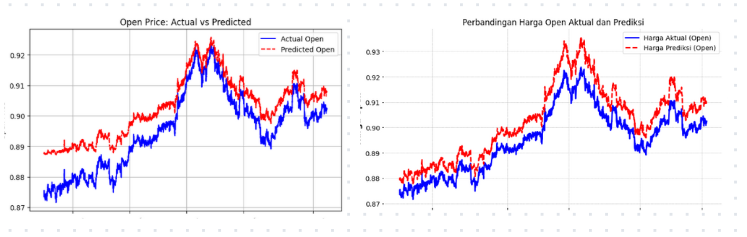
\includegraphics[scale=1.3]{gambar/perbandingan harga open(12).png} 
    \caption{Hasil Prediksi Harga Open Dengan Time Step 12}
    \label{fig:label_gambar}
\end{figure}
Pada grafik sebelah kanan, ditampilkan hasil prediksi harga open menggunakan model Time Series Transformer. Sama seperti sebelumnya, garis biru menunjukkan harga aktual dan garis merah menunjukkan hasil prediksi.Dari grafik tersebut, terlihat bahwa model Time Series Transformer mampu mengikuti pola pergerakan harga aktual. Jarak antara hasil prediksi dan harga aktual cenderung lebih konstan.Time Series Transformer menunjukkan kemampuan generalisasi yang lebih baik dalam memprediksi harga open, dengan hasil prediksi yang lebih dekat ke harga aktual dibandingkan LSTM. Hal ini sejalan dengan karakteristik Transformer yang lebih efektif dalam menangkap dependensi jangka panjang antar data time series.

\subsection{Hasil Prediksi Harga Close Dengan Timestep 12}
Hasil prediksi harga close dari model LSTM dan Time Series Transformer ditampilkan pada Gambar 4.5 berikut.
\begin{figure} [H] \centering
  % Nama dari file gambar yang diinputkan
    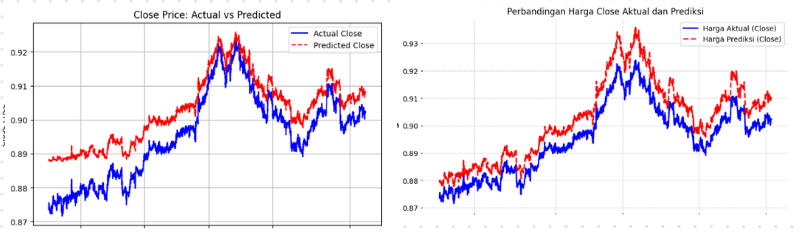
\includegraphics[scale=1.1]{gambar/perbandingan close(12).png} 
    \caption{Hasil Prediksi Harga Close Dengan Time Step 12}
    \label{fig:label_gambar}
\end{figure}

Pada grafik sebelah kiri, ditunjukkan hasil prediksi harga close menggunakan model LSTM. Garis biru menunjukkan harga aktual, sedangkan garis merah merepresentasikan hasil prediksi. Secara keseluruhan, model LSTM berhasil mengikuti arah tren pergerakan harga dengan cukup baik, baik pada fase kenaikan, puncak, maupun penurunan harga.Namun, terdapat selisih nilai yang cukup konsisten di bawah harga aktual sepanjang periode prediksi. Pola prediksi cenderung underestimate terhadap harga aktual, meskipun tren pergerakan sudah selaras. Hal ini serupa dengan pola yang terlihat pada hasil prediksi harga open, di mana LSTM mampu mengikuti tren tetapi kurang presisi dalam memprediksi nilai absolut harga.

Pada grafik sebelah kanan, ditampilkan hasil prediksi harga close menggunakan Time Series Transformer. Garis biru tetap merepresentasikan harga aktual, dan garis merah menunjukkan hasil prediksi.Dari grafik tersebut dapat dilihat bahwa model Time Series Transformer mampu mengikuti tren harga aktual dengan lebih baik, baik dari segi pola pergerakan maupun jarak antara hasil prediksi dan harga aktual. Selisih antara harga prediksi dan harga aktual relatif lebih kecil dibandingkan model LSTM, khususnya pada saat tren mengalami kenaikan maupun penurunan tajam.

\subsection{Hasil Prediksi Harga Open Dengan Timestep 24}
Hasil prediksi harga open dari Model TST dan LSTM ditampilkan pada Gambar 4.6 berikut.


\begin{figure} [H] \centering
  % Nama dari file gambar yang diinputkan
    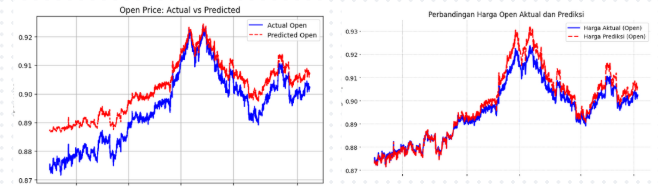
\includegraphics[scale=1.3]{gambar/perbandingan open(24).png} 
    \caption{Hasil Prediksi Harga Open Dengan Timestep 24}
    \label{fig:label_gambar}
\end{figure}

Pada grafik sebelah kiri, ditunjukkan hasil prediksi harga open menggunakan model LSTM dengan timestep 24. Seperti grafik sebelumnya, garis biru merepresentasikan harga aktual dan garis merah menunjukkan hasil prediksi.Secara pola, model LSTM mampu mengikuti arah tren pergerakan harga dengan cukup baik, baik saat tren mengalami kenaikan, puncak, maupun penurunan. Namun, hasil prediksi tetap menunjukkan pola yang kurang stabil di mana terdapat prediksi yang mempunyai jarak cukup dekat dan juga ada prediksi yang mempunyai jarak cukup jauh dari harga prediksinya.

Pada grafik sebelah kanan, ditampilkan hasil prediksi harga open menggunakan TST dengan timestep 24.Dari grafik ini, terlihat bahwa Time Series Transformer dapat mengikuti pergerakan tren harga lebih rapat dan stabil dibandingkan LSTM. Perbedaan nilai antara harga aktual dan prediksi lebih kecil, khususnya pada saat tren mengalami kenaikan maupun penurunan drastis. Selain itu, hasil prediksi Time Series Transformer tidak hanya mampu mengikuti tren, tetapi juga mendekati nilai absolut harga aktual dengan lebih baik.Jika dibandingkan dengan hasil pada timestep 12, akurasi prediksi model ini mengalami peningkatan, dengan pola pergerakan yang lebih halus dan selisih antara harga aktual dan prediksi yang lebih kecil di hampir seluruh rentang waktu.

\subsection{Hasil Prediksi Harga Close Dengan Timestep 24}
Hasil prediksi harga close dari model LSTM sebelah kiri dan model TST sebelah kanan ditampilkan pada Gambar 4.7 berikut.

\begin{figure} [H] \centering
  % Nama dari file gambar yang diinputkan
    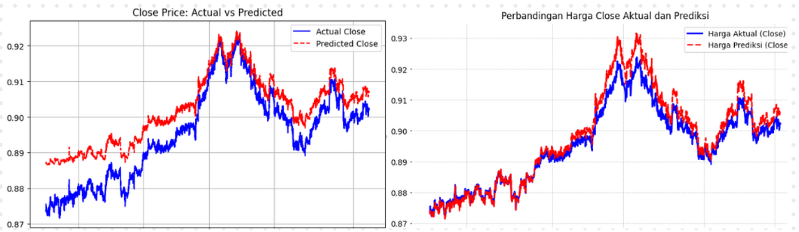
\includegraphics[scale=1.1]{gambar/perbandingan close(24).png} 
    \caption{Hasil Prediksi Harga Close Dengan Timestep 24}
    \label{fig:label_gambar}
\end{figure}
Hasil prediksi harga close mempunyai pola yang tidak berbeda jauh dengan prediksi harga open, dimana model LSTM menghasilkan prediksi yang kurang baik di awal tetapi dapat memprediksi hasil yang cukup baik di pertengahan hingga ke akhir. Sementara, model TST memprediksi hasil yang sangat baik pada timestep 24 yang di mana hasil prediksinya lebih baik dan akurat dibanding Timestep 12, terlihat secara visual bahwa hasil prediksi dari TST dapat mempertahankan jarak yang cenderung rapat dengan harga aktualnya, dan dapat memprediksi pola harga dengan baik. 

\subsection{Hasil Prediksi Harga Open Dengan Timestep 36}
Hasil prediksi harga open dari model TST dan LSTM ditampilkan pada Gambar 4.8 berikut.
\begin{figure} [H] \centering
  % Nama dari file gambar yang diinputkan
    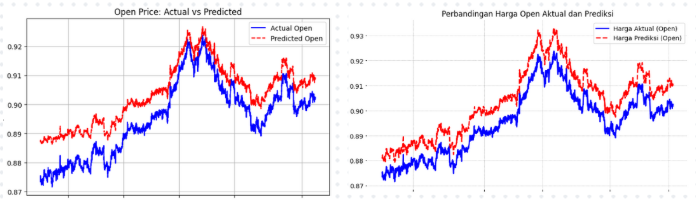
\includegraphics[scale=1.2]{gambar/perbandingan open(36).png} 
    \caption{Perbandingan Harga Open Dengan Time Step 36}
    \label{fig:label_gambar}
\end{figure}
Pada grafik sebelah kiri ditampilkan hasil prediksi dengan model LSTM, Hasil menunjukkan prediksi yang cenderung sama dengan timestep 12 dan 24 yang di mana pola maasih kurang stabil di bagian awal lalu pertengahan sampai akhir menunjukkan hasil yang cukup baik. Hasil Prediksi LSTM tergolong fluktuatif, karena jarak antara hasil aktual dan prediksi berubah ubah pada bagian awal, pertengahan hingga akhir. Sedangkan Hasil prediksi LSTM tergolong cukup baik, hasil prediksi dengan timestep 36 mempunyai kemiripan dengan hasil prediksi dengan timestep 12, tetapi jarak antar hasil prediksi dan aktual dengan timestep 36 lebih besar daripada timestep 12.

\subsection{Hasil Prediksi Harga Close Dengan Timestep 36}
Hasil prediksi harga close dari model LSTM sebelah kiri dan TST sebelah kanan dtiampilkan pada Gambar 4.9 berikut.
\begin{figure} [H] \centering
  % Nama dari file gambar yang diinputkan
    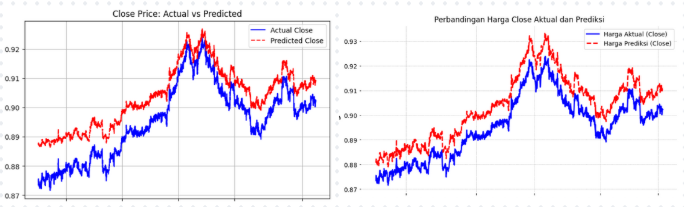
\includegraphics[scale=1.3]{gambar/perbandingan close(36).png} 
    \caption{Perbandingan Harga Close Dengan Time Step 36}
    \label{fig:label_gambar}
\end{figure}

Dari grafik tersebut dapat dilihat bahwa model LSTM masih mampu mengikuti pola tren pergerakan harga dengan cukup baik, khususnya saat terjadi tren naik dan tren turun. Namun, dibandingkan dengan timestep 24, hasil prediksi pada timestep 36 ini cenderung kurang responsif terhadap perubahan harga yang cepat, sehingga terdapat beberapa keterlambatan dalam mengikuti lonjakan harga, khususnya saat terjadi kenaikan puncak.
Time Series Transformer tetap menunjukkan performa yang lebih baik dibandingkan LSTM pada timestep 36 ini. Pola pergerakan harga berhasil diikuti dengan lebih presisi, baik saat harga mengalami tren naik, puncak, maupun penurunan.Jika dibandingkan dengan hasil prediksi Transformer pada timestep 24, performa model pada timestep 36 ini sedikit lebih stabil namun kurang tajam saat mengikuti lonjakan harga secara cepat. Meskipun demikian, selisih antara harga aktual dan prediksi tetap lebih kecil dibandingkan model LSTM, sehingga Transformer masih unggul dalam hal presisi nilai dan pola tren.
\subsection{Hasil Prediksi Open,High,Low,Close }
Pada sub bab ini akan ditampilkan hasil prediksi open, high, low, dan close tiap timestep.

\subsubsection{Hasil Prediksi Menggunakan Time Series Transformer}

\begin{figure} [H] \centering
  % Nama dari file gambar yang diinputkan
    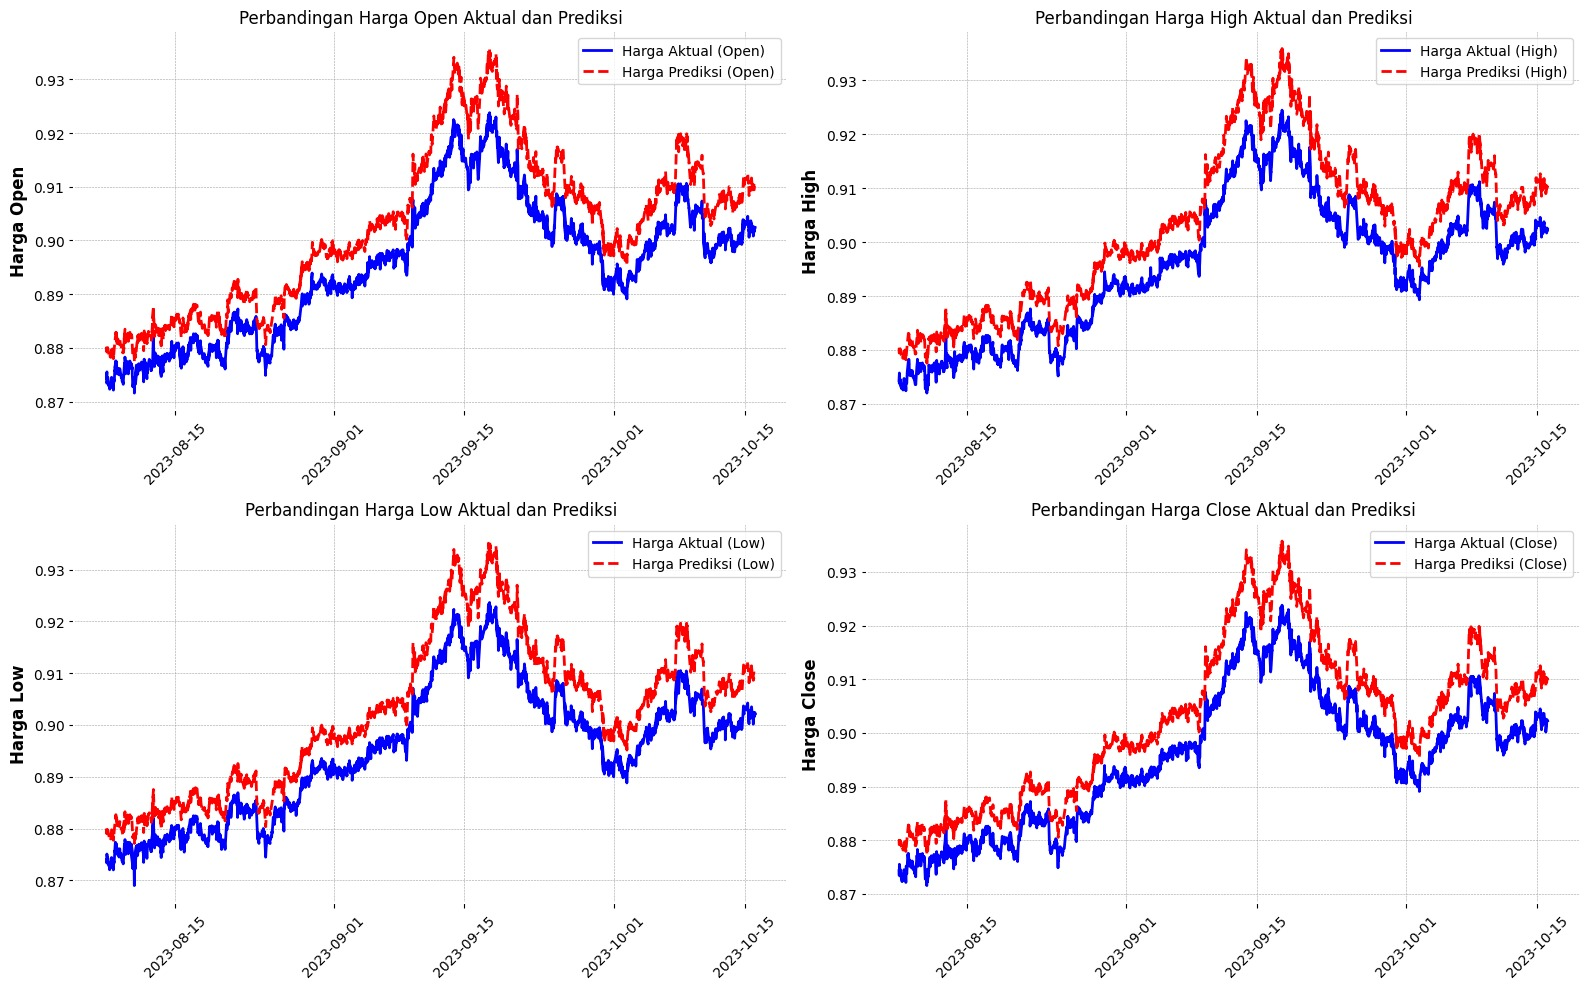
\includegraphics[scale=0.27]{gambar/perbandingan(12).png} 
    \caption{Hasil Prediksi TST Dengan Time Step 12}
    \label{fig:label_gambar}
\end{figure}
\begin{figure} [H] \centering
  % Nama dari file gambar yang diinputkan
    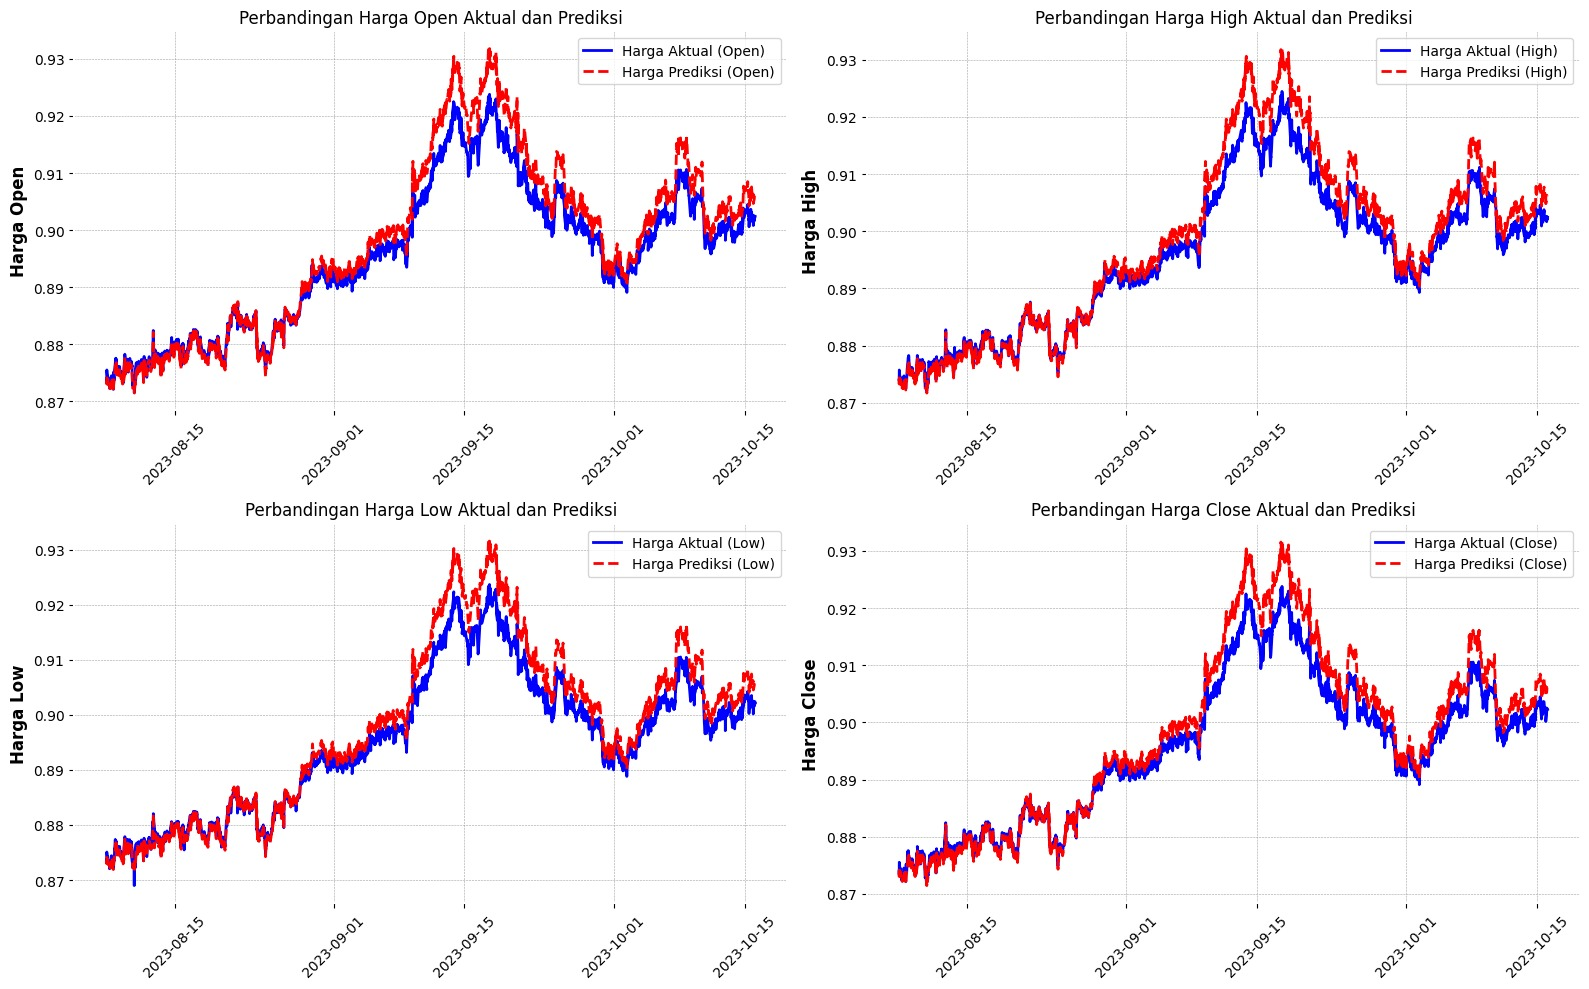
\includegraphics[scale=0.27]{gambar/perbandingan(24).png} 
    \caption{Hasil Prediksi TST Dengan Time Step 24}
    \label{fig:label_gambar}
\end{figure}
\begin{figure} [H] \centering
  % Nama dari file gambar yang diinputkan
    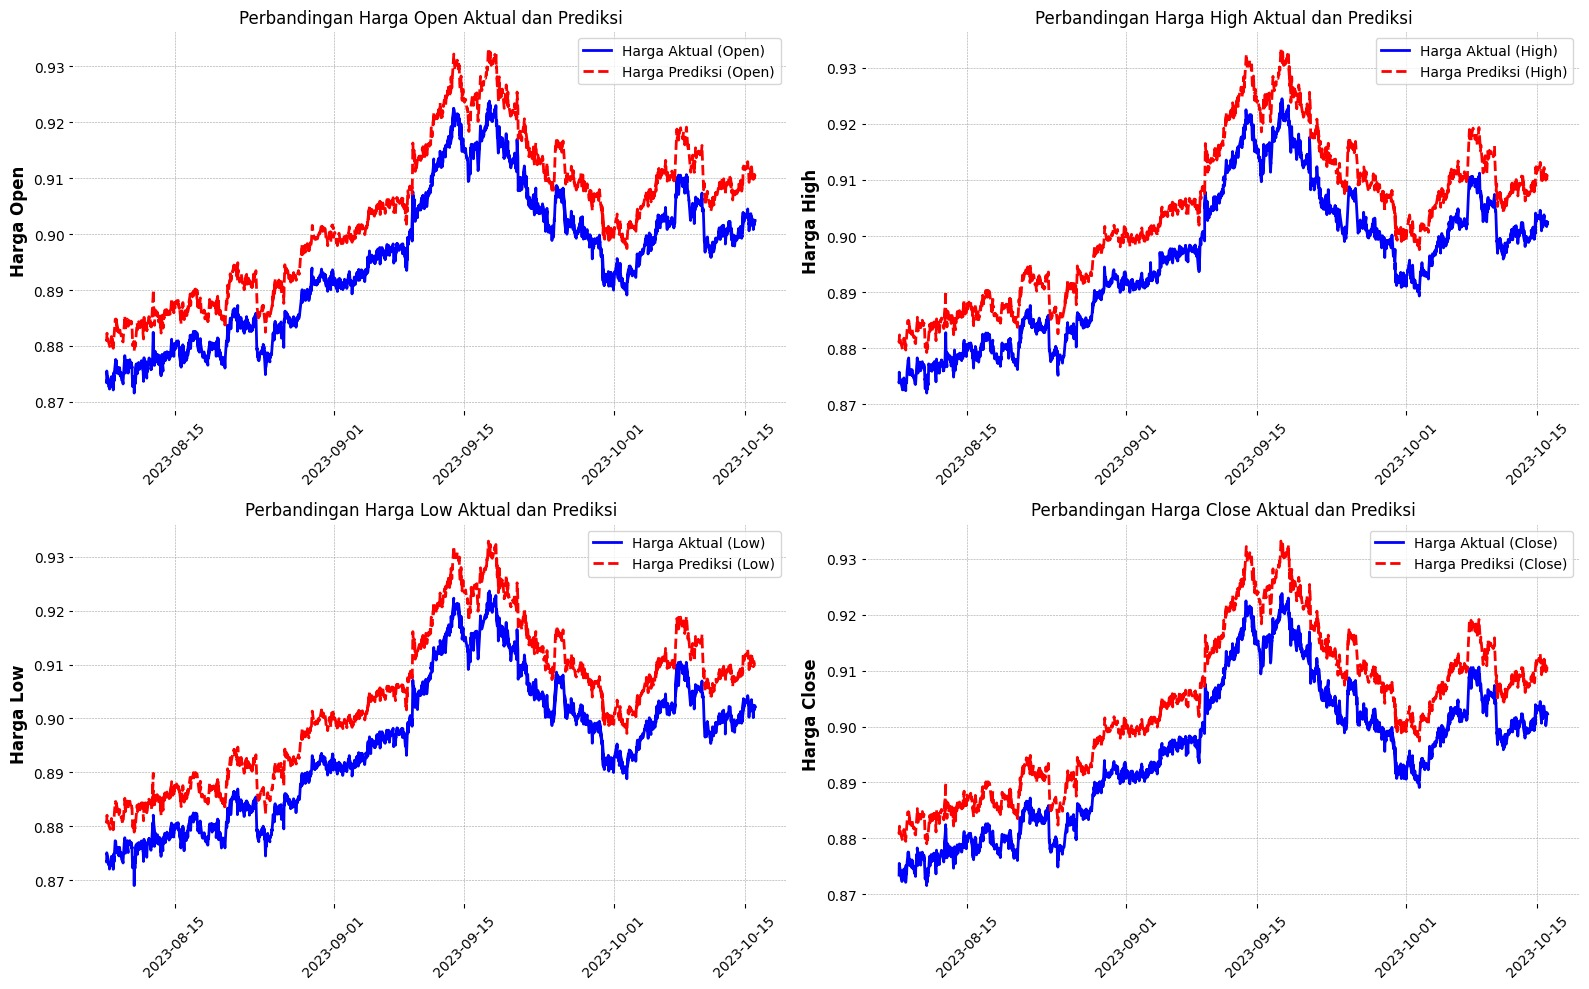
\includegraphics[scale=0.28]{gambar/perbandingan(36).png} 
    \caption{Hasil Prediksi TST Dengan Time Step 36}
    \label{fig:label_gambar}
\end{figure}

\subsubsection{Hasil Prediksi Menggunakan LSTM}
\begin{figure} [H] \centering
  % Nama dari file gambar yang diinputkan
    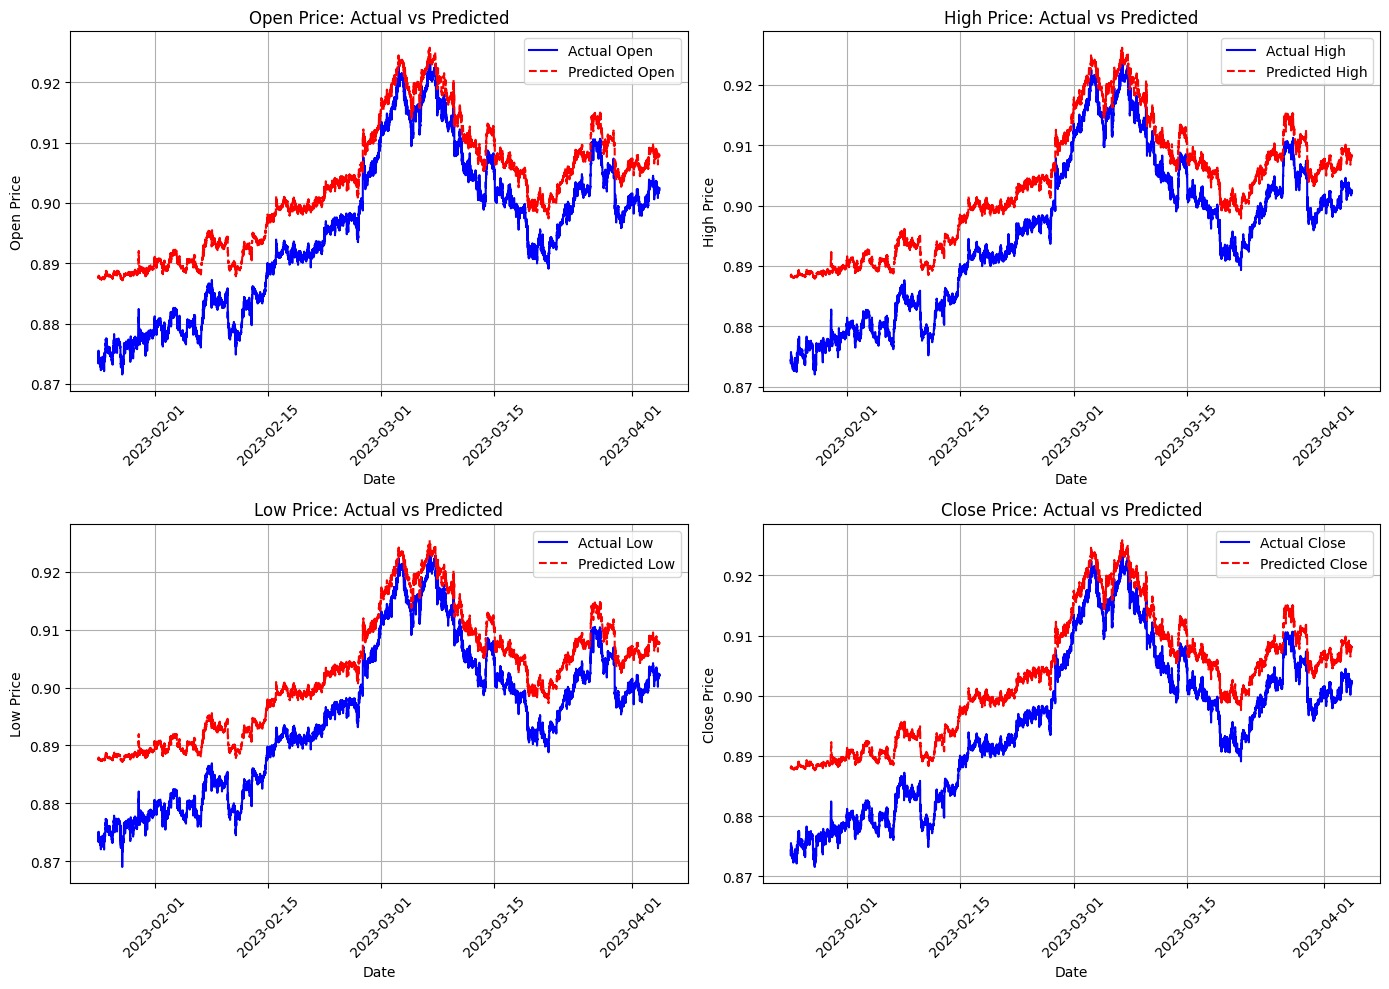
\includegraphics[scale=0.28]{gambar/hasillstm12.png} 
    \caption{Hasil Prediksi LSTM Dengan Time Step 12}
    \label{fig:label_gambar}
\end{figure}
\begin{figure} [H] \centering
  % Nama dari file gambar yang diinputkan
    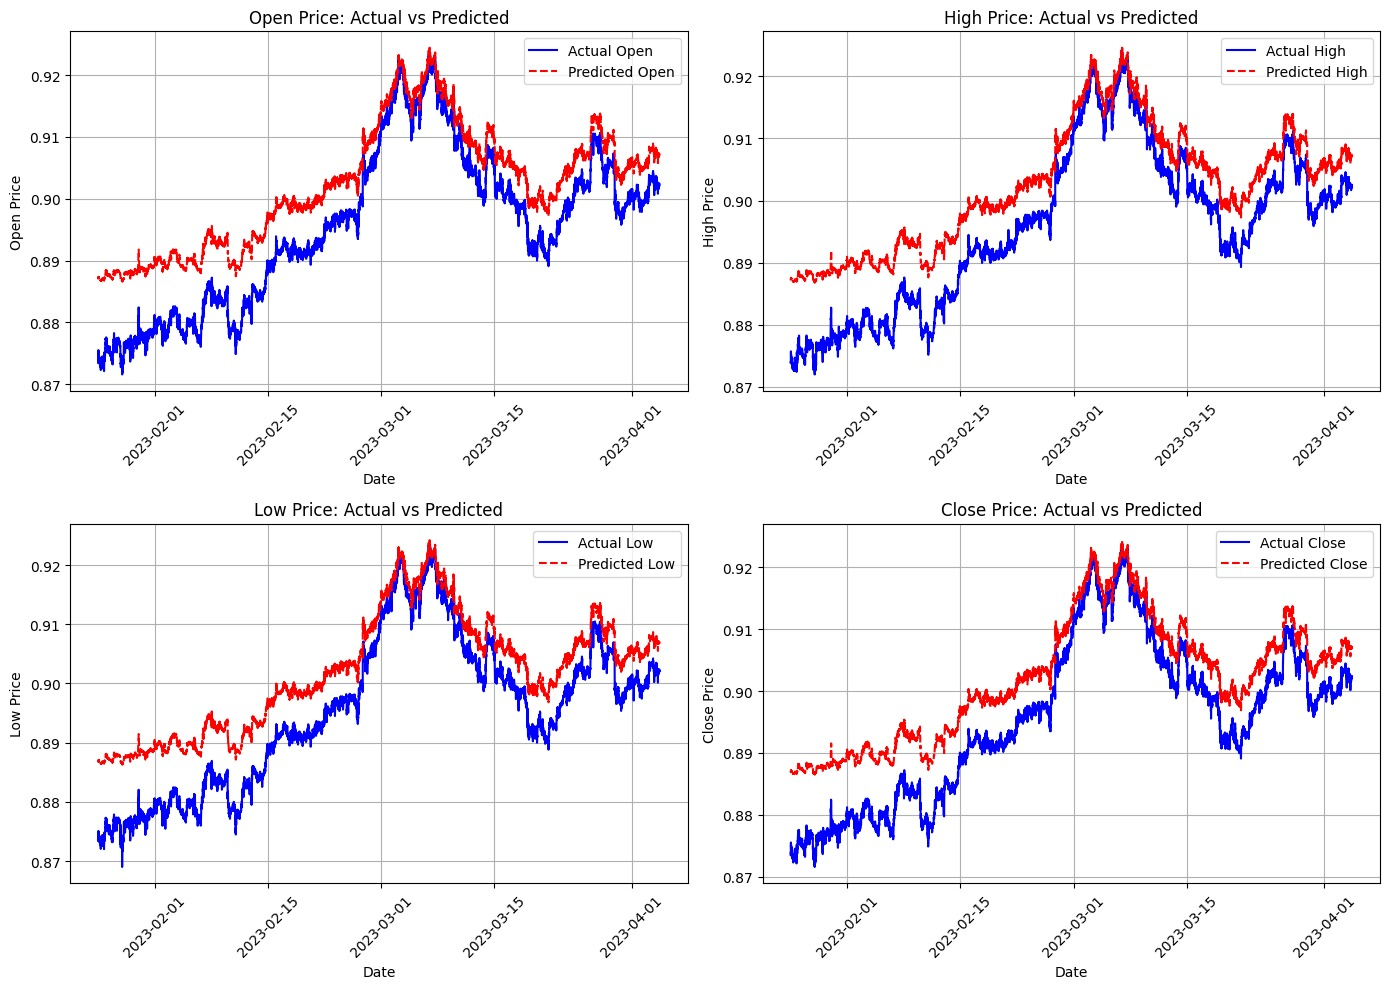
\includegraphics[scale=0.28]{gambar/hasillstm24.png} 
    \caption{Hasil Prediksi LSTM Dengan Time Step 24}
    \label{fig:label_gambar}
\end{figure}
\begin{figure} [H] \centering
  % Nama dari file gambar yang diinputkan
    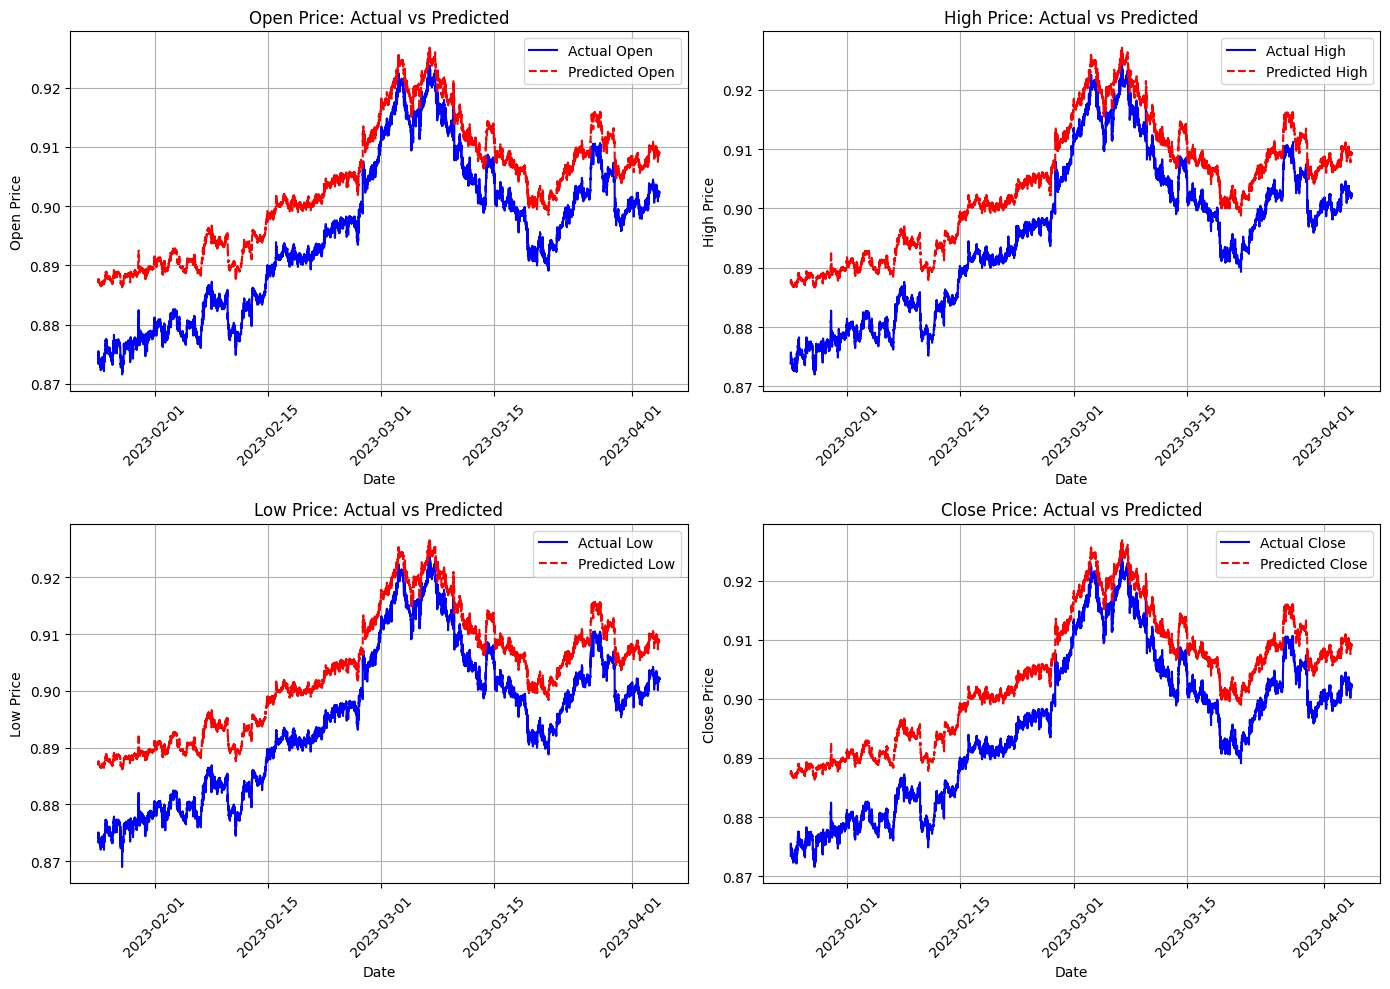
\includegraphics[scale=0.28]{gambar/hasillstm36.png} 
    \caption{Hasil Prediksi LSTM Dengan Time Step 36}
    \label{fig:label_gambar}
\end{figure}


Berdasarkan hasil pengujian model Time Series Transformer dengan variasi timestep 12, 24, dan 36, dapat dianalisis bahwa timestep 24 mempunyai prediksi yang lebih baik dari yang lain. Hal ini terlihat dari keselarasan antara grafik prediksi (warna merah) dan grafik aktual (warna biru), khususnya pada parameter Close dan Low , di mana prediksi model mampu mengikuti tren pergerakan harga secara cukup akurat. Pada timestep 12, model menunjukkan performa yang cukup baik, tetapi masih terdapat beberapa deviasi terutama pada fluktuasi harga yang tajam. Pada time step 36, model menunjukkan performa yang cukup baik, tetapi masih terdapat jarak antara harga aktual dan prediksi, dan menjadi yang paling buruk diantara yang lainnya. Timestep 24 memberikan hasil terbaik dibandingkan dua timestep lainnya, di mana prediksi lebih stabil dan mendekati harga aktual, meskipun tetap terdapat sedikit penyimpangan pada perubahan harga yang mendadak. Secara visual, model dengan timestep 24 memiliki stabilitas dan ketepatan tren yang lebih baik, sehingga dapat dikatakan sebagai konfigurasi optimal dalam pengujian ini.

Berdasarkan pengujian model LSTM dengan timestep 12,24, dan 36, secara visual didapatkan hasil yang cukup baik untuk prediksi dan tidak berbeda jauh di timestep 12,24,dan 36 di mana prediksi bisa memprediksi kenaikan dan penurunan yang signifikan, tetapi hasil prediksi kurang stabil karena untuk hasil awal jarak yang terdapat antara harga aktual dan prediksi cukup jauh dan saat pertengahan sampai akhir hasil prediksi megnhasilkan jarak yang cukup dekat antara harga prediksi dan harga aktual.


\subsection{Hasil Prediksi menggunakan data real-time pada Model Time Series Transformer dan LSTM}

Dilakukan pengujian model dengan data real-time yang diambil dari situs Investing.com. Data yang digunakan adalah data blablabla dengan interval 5 menit selama 1000 data terakhir. Hasil prediksi menggunakan model Time Series Transformer dan LSTM ditampilkan pada Grafik menggunakan libary matplotlib dan mplfinance. 

\subsubsection*{4.3.8.1 Hasil Prediksi Menggunakan Time Series Transformer}
Model yang digunakan yaitu model Time Series Transformer dengan timestep 24. Hasil prediksi ditampilkan pada Gambar \ref{fig:label_gambar} berikut.
% \begin{figure}

% \end{figure}

Dari hasil yang didapatkan menggunakan akun demo didapatkan dari 30 kali transaksi, didapatkan sekian transaksi profit dan transaksi loss, dengan total profit sekian dan total loss sekian. Dengan rata-rata profit sekian dan rata-rata loss sekian. Dengan persentase profit sekian persen dan persentase loss sekian persen. Dengan rasio profitabilitas sekian persen.

sehingga bisa didapatkan tabel ref yang merupakan masing masing profit dan loss yang didapatkan. 

\begin{table}[H]
  \centering
  \begin{tabular}{|c|c|l|l|l|l|l|}
  \cline{1-3} \cline{5-7}
  \textit{Percobaan}     & \textit{Profit}       & \textit{Loss} &  & \multicolumn{1}{c|}{\textit{Percobaan}} & \multicolumn{1}{c|}{\textit{Profit}} & \textit{Loss} \\ \cline{1-3} \cline{5-7} 
                         &                       &               &  &                                         &                                      &               \\ \cline{1-3} \cline{5-7} 
                         &                       &               &  &                                         &                                      &               \\ \cline{1-3} \cline{5-7} 
                         &                       &               &  &                                         &                                      &               \\ \cline{1-3} \cline{5-7} 
                         &                       &               &  &                                         &                                      &               \\ \cline{1-3} \cline{5-7} 
                         &                       &               &  &                                         &                                      &               \\ \cline{1-3} \cline{5-7} 
                         &                       &               &  &                                         &                                      &               \\ \cline{1-3} \cline{5-7} 
                         &                       &               &  &                                         &                                      &               \\ \cline{1-3} \cline{5-7} 
                         &                       &               &  &                                         &                                      &               \\ \cline{1-3} \cline{5-7} 
                         &                       &               &  &                                         &                                      &               \\ \cline{1-3} \cline{5-7} 
                         &                       &               &  &                                         &                                      &               \\ \cline{1-3} \cline{5-7} 
  \multicolumn{1}{|l|}{} & \multicolumn{1}{l|}{} &               &  &                                         &                                      &               \\ \cline{1-3} \cline{5-7} 
  \multicolumn{1}{|l|}{} & \multicolumn{1}{l|}{} &               &  &                                         &                                      &               \\ \cline{1-3} \cline{5-7} 
  \multicolumn{1}{|l|}{} & \multicolumn{1}{l|}{} &               &  &                                         &                                      &               \\ \cline{1-3} \cline{5-7} 
  \multicolumn{1}{|l|}{} & \multicolumn{1}{l|}{} &               &  &                                         &                                      &               \\ \cline{1-3} \cline{5-7} 
  \multicolumn{1}{|l|}{} & \multicolumn{1}{l|}{} &               &  &                                         &                                      &               \\ \cline{1-3} \cline{5-7} 
  \end{tabular}
  \end{table}


\begin{table}[H]
  \centering
    \begin{tabular}{|c|c|l|}
    \hline
    \textit{Percobaan} & \textit{Average Profit} & \textit{Average Loss} \\ \hline
                       &                         &                       \\ \hline
    \end{tabular}
\end{table}

\subsubsection*{4.3.8.2 Hasil Prediksi Menggunakan LSTM}
Model yang digunakan yaitu model LSTM Model Pertama dengan timestep 24. Hasil prediksi ditampilkan pada Gambar \ref{fig:label_gambar} berikut.
% \begin{figure}

% \end{figure}

Dari hasil yang didapatkan menggunakan akun demo didapatkan dari 30 kali transaksi, didapatkan sekian transaksi profit dan transaksi loss, dengan total profit sekian dan total loss sekian. Dengan rata-rata profit sekian dan rata-rata loss sekian. Dengan persentase profit sekian persen dan persentase loss sekian persen. Dengan rasio profitabilitas sekian persen.

sehingga bisa didapatkan tabel ref yang merupakan masing masing profit dan loss yang didapatkan. 

\begin{table}[H]
  \centering
  \begin{tabular}{|c|c|l|l|l|l|l|}
  \cline{1-3} \cline{5-7}
  \textit{Percobaan}     & \textit{Profit}       & \textit{Loss} &  & \multicolumn{1}{c|}{\textit{Percobaan}} & \multicolumn{1}{c|}{\textit{Profit}} & \textit{Loss} \\ \cline{1-3} \cline{5-7} 
                         &                       &               &  &                                         &                                      &               \\ \cline{1-3} \cline{5-7} 
                         &                       &               &  &                                         &                                      &               \\ \cline{1-3} \cline{5-7} 
                         &                       &               &  &                                         &                                      &               \\ \cline{1-3} \cline{5-7} 
                         &                       &               &  &                                         &                                      &               \\ \cline{1-3} \cline{5-7} 
                         &                       &               &  &                                         &                                      &               \\ \cline{1-3} \cline{5-7} 
                         &                       &               &  &                                         &                                      &               \\ \cline{1-3} \cline{5-7} 
                         &                       &               &  &                                         &                                      &               \\ \cline{1-3} \cline{5-7} 
                         &                       &               &  &                                         &                                      &               \\ \cline{1-3} \cline{5-7} 
                         &                       &               &  &                                         &                                      &               \\ \cline{1-3} \cline{5-7} 
                         &                       &               &  &                                         &                                      &               \\ \cline{1-3} \cline{5-7} 
  \multicolumn{1}{|l|}{} & \multicolumn{1}{l|}{} &               &  &                                         &                                      &               \\ \cline{1-3} \cline{5-7} 
  \multicolumn{1}{|l|}{} & \multicolumn{1}{l|}{} &               &  &                                         &                                      &               \\ \cline{1-3} \cline{5-7} 
  \multicolumn{1}{|l|}{} & \multicolumn{1}{l|}{} &               &  &                                         &                                      &               \\ \cline{1-3} \cline{5-7} 
  \multicolumn{1}{|l|}{} & \multicolumn{1}{l|}{} &               &  &                                         &                                      &               \\ \cline{1-3} \cline{5-7} 
  \multicolumn{1}{|l|}{} & \multicolumn{1}{l|}{} &               &  &                                         &                                      &               \\ \cline{1-3} \cline{5-7} 
  \end{tabular}
  \end{table}


\begin{table}[H]
  \centering
    \begin{tabular}{|c|c|l|}
    \hline
    \textit{Percobaan} & \textit{Average Profit} & \textit{Average Loss} \\ \hline
                       &                         &                       \\ \hline
    \end{tabular}
\end{table}

\subsubsection*{4.3.8.3 Hasil Prediksi Menggunakan LSTM Model 2}
Model yang digunakan yaitu model LSTM Arsitektur 2 dengan timestep 24. Hasil prediksi ditampilkan pada Gambar \ref{fig:label_gambar} berikut.
% \begin{figure}

% \end{figure}

Dari hasil yang didapatkan menggunakan akun demo didapatkan dari 30 kali transaksi, didapatkan sekian transaksi profit dan transaksi loss, dengan total profit sekian dan total loss sekian. Dengan rata-rata profit sekian dan rata-rata loss sekian. Dengan persentase profit sekian persen dan persentase loss sekian persen. Dengan rasio profitabilitas sekian persen.

sehingga bisa didapatkan tabel ref yang merupakan masing masing profit dan loss yang didapatkan. 

\begin{table}[H]
  \centering
  \begin{tabular}{|c|c|l|l|l|l|l|}
  \cline{1-3} \cline{5-7}
  \textit{Percobaan}     & \textit{Profit}       & \textit{Loss} &  & \multicolumn{1}{c|}{\textit{Percobaan}} & \multicolumn{1}{c|}{\textit{Profit}} & \textit{Loss} \\ \cline{1-3} \cline{5-7} 
                         &                       &               &  &                                         &                                      &               \\ \cline{1-3} \cline{5-7} 
                         &                       &               &  &                                         &                                      &               \\ \cline{1-3} \cline{5-7} 
                         &                       &               &  &                                         &                                      &               \\ \cline{1-3} \cline{5-7} 
                         &                       &               &  &                                         &                                      &               \\ \cline{1-3} \cline{5-7} 
                         &                       &               &  &                                         &                                      &               \\ \cline{1-3} \cline{5-7} 
                         &                       &               &  &                                         &                                      &               \\ \cline{1-3} \cline{5-7} 
                         &                       &               &  &                                         &                                      &               \\ \cline{1-3} \cline{5-7} 
                         &                       &               &  &                                         &                                      &               \\ \cline{1-3} \cline{5-7} 
                         &                       &               &  &                                         &                                      &               \\ \cline{1-3} \cline{5-7} 
                         &                       &               &  &                                         &                                      &               \\ \cline{1-3} \cline{5-7} 
  \multicolumn{1}{|l|}{} & \multicolumn{1}{l|}{} &               &  &                                         &                                      &               \\ \cline{1-3} \cline{5-7} 
  \multicolumn{1}{|l|}{} & \multicolumn{1}{l|}{} &               &  &                                         &                                      &               \\ \cline{1-3} \cline{5-7} 
  \multicolumn{1}{|l|}{} & \multicolumn{1}{l|}{} &               &  &                                         &                                      &               \\ \cline{1-3} \cline{5-7} 
  \multicolumn{1}{|l|}{} & \multicolumn{1}{l|}{} &               &  &                                         &                                      &               \\ \cline{1-3} \cline{5-7} 
  \multicolumn{1}{|l|}{} & \multicolumn{1}{l|}{} &               &  &                                         &                                      &               \\ \cline{1-3} \cline{5-7} 
  \end{tabular}
  \end{table}


\begin{table}[H]
  \centering
    \begin{tabular}{|c|c|l|}
    \hline
    \textit{Percobaan} & \textit{Average Profit} & \textit{Average Loss} \\ \hline
                       &                         &                       \\ \hline
    \end{tabular}
\end{table}

\subsubsection*{4.3.8.4 Hasil Prediksi Menggunakan LSTM Model 3}
Model yang digunakan yaitu model LSTM Bidirectional dengan timestep 24. Hasil prediksi ditampilkan pada Gambar \ref{fig:label_gambar} berikut.
% \begin{figure}

% \end{figure}

Dari hasil yang didapatkan menggunakan akun demo didapatkan dari 30 kali transaksi, didapatkan sekian transaksi profit dan transaksi loss, dengan total profit sekian dan total loss sekian. Dengan rata-rata profit sekian dan rata-rata loss sekian. Dengan persentase profit sekian persen dan persentase loss sekian persen. Dengan rasio profitabilitas sekian persen.

sehingga bisa didapatkan tabel ref yang merupakan masing masing profit dan loss yang didapatkan. 

\begin{table}[H]
  \centering
  \begin{tabular}{|c|c|l|l|l|l|l|}
  \cline{1-3} \cline{5-7}
  \textit{Percobaan}     & \textit{Profit}       & \textit{Loss} &  & \multicolumn{1}{c|}{\textit{Percobaan}} & \multicolumn{1}{c|}{\textit{Profit}} & \textit{Loss} \\ \cline{1-3} \cline{5-7} 
                         &                       &               &  &                                         &                                      &               \\ \cline{1-3} \cline{5-7} 
                         &                       &               &  &                                         &                                      &               \\ \cline{1-3} \cline{5-7} 
                         &                       &               &  &                                         &                                      &               \\ \cline{1-3} \cline{5-7} 
                         &                       &               &  &                                         &                                      &               \\ \cline{1-3} \cline{5-7} 
                         &                       &               &  &                                         &                                      &               \\ \cline{1-3} \cline{5-7} 
                         &                       &               &  &                                         &                                      &               \\ \cline{1-3} \cline{5-7} 
                         &                       &               &  &                                         &                                      &               \\ \cline{1-3} \cline{5-7} 
                         &                       &               &  &                                         &                                      &               \\ \cline{1-3} \cline{5-7} 
                         &                       &               &  &                                         &                                      &               \\ \cline{1-3} \cline{5-7} 
                         &                       &               &  &                                         &                                      &               \\ \cline{1-3} \cline{5-7} 
  \multicolumn{1}{|l|}{} & \multicolumn{1}{l|}{} &               &  &                                         &                                      &               \\ \cline{1-3} \cline{5-7} 
  \multicolumn{1}{|l|}{} & \multicolumn{1}{l|}{} &               &  &                                         &                                      &               \\ \cline{1-3} \cline{5-7} 
  \multicolumn{1}{|l|}{} & \multicolumn{1}{l|}{} &               &  &                                         &                                      &               \\ \cline{1-3} \cline{5-7} 
  \multicolumn{1}{|l|}{} & \multicolumn{1}{l|}{} &               &  &                                         &                                      &               \\ \cline{1-3} \cline{5-7} 
  \multicolumn{1}{|l|}{} & \multicolumn{1}{l|}{} &               &  &                                         &                                      &               \\ \cline{1-3} \cline{5-7} 
  \end{tabular}
  \end{table}


\begin{table}[H]
  \centering
    \begin{tabular}{|c|c|l|}
    \hline
    \textit{Percobaan} & \textit{Average Profit} & \textit{Average Loss} \\ \hline
                       &                         &                       \\ \hline
    \end{tabular}
\end{table}

\section{Evaluasi Pengujian}
\label{sec:analisispengujian}

Dari pengujian yang \lipsum[1]

% Contoh pembuatan tabel
\begin{longtable}{|c|c|c|}
  \caption{Hasil Pengukuran Energi dan Kecepatan}
  \label{tb:EnergiKecepatan}                                   \\
  \hline
  \rowcolor[HTML]{C0C0C0}
  \textbf{Energi} & \textbf{Jarak Tempuh} & \textbf{Kecepatan} \\
  \hline
  10 J            & 1000 M                & 200 M/s            \\
  20 J            & 2000 M                & 400 M/s            \\
  30 J            & 4000 M                & 800 M/s            \\
  40 J            & 8000 M                & 1600 M/s           \\
  \hline
\end{longtable}

\lipsum[2-4]
